\documentclass[a4paper,12pt, twoside]{article}
%layout packages
\usepackage{geometry} %Page layout
\geometry{a4paper, top=25mm, left=25mm, right=25mm, bottom=25mm,
         headsep=10mm, footskip=12mm}
\usepackage{lscape}
\usepackage{setspace} %linespacings
\onehalfspacing
\usepackage{graphicx}
\usepackage{color}
\usepackage{textcomp} %Celsius symbol, euro sign
\usepackage{amsmath} %formula
\usepackage{mathtools} %formula
\usepackage{amssymb}
\usepackage{url}
\usepackage{xfrac}
%\usepackage{showkeys} %zeigt keys der Bilder an, vor Endversion auskommentieren
\usepackage{listings} % f\"{u}r source code formatting
	\lstset{language=R,
		basicstyle=\footnotesize
		}
%\usepackage[toc,page]{Appendix}
\usepackage{verbatim} % enables to 'comment' entire paragraphs

% enables to run makeindex used for package{nomencl} from within latex document
\def\execute{%
\begingroup
\catcode`\%=12
\catcode`\\=12
\executeaux}
\def\executeaux#1{\immediate\write18{#1}\endgroup}
\usepackage[intoc]{nomencl}
%\execute{makeindex Masterarbeit.nlo -s nomencl.ist -o Masterarbeit.nls}
\renewcommand{\nomname}{Abbreviations} 	% changes name nomenclature to abbreviations
\setlength{\nomitemsep}{-\parsep}
\setlength{\nomlabelwidth}{.20\hsize}
\makenomenclature

%Figure packages
\usepackage{wrapfig} %erm\"{o}glicht, text um bilder flie\\ßen zu lassen
%\usepackage{subfig}
\usepackage{rotating} %damit bildunterschrift auch gedreht werden kann
\usepackage{graphicx} 
\usepackage{caption} 
\usepackage{subcaption}

%tabular packages
\usepackage{multirow}
%\usepackage{longTable}
\usepackage{array}
\usepackage{booktabs} %nice looking Tables
\usepackage[labelformat=simple, labelsep=colon, justification=justified, labelfont=bf, textfont=normalfont, font=small]{caption}
\captionsetup[lstlisting]{font=singlespacing} 

%new Table column types
\newcolumntype{R}[1]{>{\raggedleft\arraybackslash}#1}		%rechtsb\"{u}ndig
\newcolumntype{L}[1]{>{\raggedright\arraybackslash}#1}		%linksb\"{u}ndig
\newcolumntype{C}[1]{>{\centering\arraybackslash}#1}		%zentriertO


% other new commands
\newcommand{\HRule}{\rule{\textwidth}{0.5mm}}
\newcommand{\up}[1]{\ensuremath{^{\textrm{\tiny#1}}}}	% hochstellen im flie\\ßtext
\newcommand{\down}[1]{\ensuremath{_{\textrm{\tiny#1}}}}	% tiefstellen im flie\\ßtext
\newcommand{\beginsupplement}{%
        \setcounter{table}{0}
        \renewcommand{\thetable}{S\arabic{table}}%
        \setcounter{figure}{0}
        \renewcommand{\thefigure}{S\arabic{figure}}%
     }

% bib packages
\ProvidesFile{merlin.mbs}[2011/03/28 4.32 (PWD, AO, DPC)]
\usepackage{natbib}
\bibpunct{[}{]}{,}{a}{}{,}

\begin{document}
\include{TAC3_title}
\chapter{Introduction}

The field of quantitative genetics has come far since Fisher's initial studies on growth traits in wheat in 1918 \citep{}. While back then the concept of inheritance existed, little was known about the molecule responsible.  The discovery of the DNA structure by Franklin, Watson and Crick and technical break-throughs in analysing its sequence some xx years later, have allowed to investigate genetic variance on a much more detailed scale, moving from whole chromosomes and linkage studies to the analysis of DNA variation on a single-base pair level. The developments gentoyping and sequencing technologies in the recent years, have made large scale studies on genetic variation feasible. With the sinking costs of genotyping techniques, the number of samples investigated has risen and studies investigating effect of single DNA bases often comprise thousands of individuals, especially in the field of human genetics.  Together with the increased number of samples available in these studies, the number of phenotypes that are measured for each individual has grown from a few measurements to tens or even hundreds. The availability of these rich datasets provides great opportunities in studying genetic variations and its outcomes, such as studying pleiotropy and xx.  However, it also poses technical challenges in analysing these dataset. 

 Many cohort studies now have rich, high dimensional datasets ranging from studies in model organism such as yeast and arabidopsis thaliana to human molecular, morphological or imaging derived traits \citep{Bloom2013,Atwell2010,Astle2009,Shaffer2016,Stein2010}. However, these cohorts have often been analysed trait by trait partly for simplicity and partly because of a paucity of models suitable for the anlaysis of the high dimensional phenotype data.

\section{Multi-trait mapping}
Many cohort studies today, ranging from studies in model organism such as yeast and arabidopsis thaliana to human, have rich, high dimensional datasets including molecular, morphological or imaging derived traits \citep{Bloom2013,Atwell2010,Astle2009,Shaffer2016,Stein2010}. However, these traits have often been analysed separately,  partly for simplicity and partly because of a paucity of models suitable for the anlaysis of high-dimensional phenotype data. A variety of multi-trait models have been developed which can be broadly grouped into three different classes: i) dimensionality reduction techniques, ii) meta-analysis approaches and iii) multivariate regression models (reviewed in \citep{Shriner2012,Yang2012}). 
\paragraph{Dimensionality reduction techniques}  
Dimensionality reduction methods in genotype-phenotype mapping seek to find a linear combination of the phenotypes \(\mat{Y} \in \mathcal{R}^{N,P}\) into a lower dimensional space \(\tilde{\mat{Y}} \in \mathcal{R}^{N,K}\):
\begin{equation}
\tilde{\mat{Y}} = b_1\mat{y}_1 + b_2\mat{y}_2 + \dots + b_P\mat{y}_P
\end{equation}

Two commonly employed dimensionality reduction methods are principal component analysis (PCA) and canonical correlation analyses (CCA). In PCA, the components of the new phenotype representation are called principal components (PC) and are the eigenvectors \tmat{W} of the empirical covariance matrix \(\mat{Y}^T\mat{Y}\): \(\mat{Y}^T\mat{Y} = \mat{W}\mat{\Lambda}\mat{W}^T\). The eigenvalues \(\Lambda\) corresponding to the PCs are equivalent to the variance explained by their components. The transformation of the phenotype data into principal components leads to a projection where the highest amount of phenotypic variance explained lies in the first component, the second highest variance in the second component and so forth. The dimensionality reduction is achieved by using the first \(K\) principal components until the cumulative sum of the eigenvalues reaches a predefined threshold of total phenotypic variance that should be retained. These \(K\) principal components are used as proxy phenotypes for the association study. PCA as a dimensionality reduction technique has for instance been used in studies to find links between genotypes and facial features or obesity phenotypes \citep{Liu2012,Claes2014,He2008}. Recently, Aschard and colleagues \ref{Aschard2014} demonstrated that simply focusing on the principal components with the highest variance might not exploit the full potential of using PCA for genetic association. They propose a model of combined PCA where the PCs are grouped based on the level of variance they explain. They show a power gain in detecting genetic associations compared to simple approaches of only testing the top few PCs.

While the PCA dimensionality reduction approach focus on the phenotype space and subsequent association with the genotypes, CCA finds the optimal transformation of \tmat{Y} into \(\tilde{\mat{Y}}\) while simultaneously testing for the association with the genotypes. Originally proposed by Hotelling for any set of variables that remain invariant under internal linear transformation\citeyear{Hotelling1936}, in quantitative genetics CCA seeks to maximise the canonical correlation \(\hat{\rho}\) between  \(\tilde{\mat{Y}}= A^T\mat{Y}\) and a genotype \(\mat{X} \in \mathcal{R}^{N,1}\):   \(\hat{\rho} = cor(\mat{X},\tilde{\mat{Y}}) = \Sigma_{XY}A(A^T\Sigma_{YY}A\Sigma_{XX})^{-\frac{1}{2}}\). \(\Sigma_{YY},\Sigma_{XX} \text{ and } \Sigma_{XY}\) are the empirical sample covariance matrices of the phenotypes, the genotypes and cross-covariance of the phenotypes and genotypes, respectively. \(\hat{\rho}\) is maximised by finding the squared root of the largest eigenvalue of the \(\Sigma_{YY}^{-1}\Sigma_{YX}\Sigma_{XX}^{-1}\Sigma_{XY}\) covariance matrix and the corresponding eigenvector \tmat{A} contains the coefficients for constructing \(\tilde{\mat{Y}}\) \citep{Yang2102}. CCA finds the transformation \(\tilde{\mat{Y}}\) that explains the maximum amount of the covariation between the genotype and all traits. The significance of the correlation i.e. the genotype-phenotype association can be tested via Bartlett's likelihood ratio test with the null hypothesis of \(\text{H}_\text{0: }\Sigma_{YX} = 0\) \citep{Bartlett1941}. Ferreira and Purcell showed in simulations that CCA with multiple traits and one genetic marker \tmat{X} controls well for type I errors and has increased power compared to multivariate tests. In order to extend the CCA method to more than one marker, the genotypes also undergo a linear transformation: 
 \(\hat{\rho} = cor(B^T\mat{X},A^T\mat{Y}) = B^T\Sigma_{XY}A(A^T\Sigma_{YY}AB^T\Sigma_{XX}B)^{-\frac{1}{2}}\) and the maximum \(\hat{\rho}\) is found by solving for the largest eigenvalue of both \tmat{A} and \tmat{B}. As the number of genotype markers in GWAS exceeds the number of samples, estimates of the covariance matrix \(X^TX\) become unreliable \citep{Schaefer2005}. Several methods have been developed to circumvent this issue, making use of sparse matrices \citep{Parkhomenko2009} or a priori grouping of the genotypes \citep{Naylor2010}. 

 \paragraph{Meta-analysis approaches}
Meta-analysis approaches combine the simplicity of the univariate approaches with the advantages of the multivariate approach. For each phenotype, a univariate association study is conducted and the summary stastics of these tests combined. Many methods for combining the summary statistics \citep{Xu2003,Yang2010,Yang2012,Bolormaa2014} go back to the work by O'Brien \citep{O'Brien1984}, who proposed to use a linear combination of the observed test statistics for each univariate test \(\mat{T} =(T_1, \dots, T_P)^T\) as the new statistics to be evaluated for significance.  \tmat{T} is asymptoctically normal distributed with mean \(\mat{\mu} = (\mu_1,\ldots, \mu_P)^T\) and covariance matrix \(\mat{\Sigma}\). O'Brien stastistic allows for testing the Null hypothesis \(H_0: \mu = 0\) against the alternative hypothesis of  \(H_1: \mu_p \ge 0, p=1, \ldots , P \) and is most powerful if \(\mu_1= \ldots =\mu_P\) \citep{Xu2003}. It is defined as: \(S = \mat{J}^T \mat{\Sigma}\mat{T}\), with \(\mat{J} = (1, 1, \ldots, 1)^T\).  The statistic has been modified in a number of studies, by adapting either the weighting matrix \tmat{J}, the covariance matrix \tmat{\Sigma} or both. Xu and colleagues \citeyear{Xu2003} optimised \(S\) to allow for testing against a general \(\mu\) rather then for a case where  \(\mu_1= \ldots =\mu_P\) by allowing for flexible, but restrained weights in \tmat{J}. Similarily, Yang and colleagues  \citeyear{Yang2010} proposed non-uniform weights to reflect heterogeneity in the means and use a sample splitting and cross-validation approach to determine the optimal weights. 
While the previous two studies showed an increase in power for using the combined statistic, they either used a small marker set or small number of phenotypic traits.  Bolormaa and colleagues showed that these power gains also hold for genotype to phenotype mapping of 32 traits across all genome-wide markers \citep{Bolormaa2014}. In their study, the weights of O'Briens proposal are substituted by the signed t-statistic. 

\paragraph{Regression models} There are a number of different regression models that allow for the multivariate analysis of phenotypes. Among them are graphical models, generalized estimation equations and frailty models, for which a summary of methods and application can be found in \citep{Shriner2012,Yang2012}. Here, I will focus on describing the development of multivariate linear regression models for genotype-phenotype mapping. The underlying models and their derivation have been described in \cref{sec:intro}. Before the era of GWAS, QTL mapping in linkage experiments have demonstrated the increase in power when jointly analysing traits with common underlying genetics. Jiang and colleagues \citeyearpar{Jiang1995} proposed a multi-trait model where the phenotypes are jointly modeled as the sum of the fixed genetic effects of interest, fixed effects for genetic background variation and residual noise. They show that the joint analysis of traits can increase power to detect the underlying genetics and can increase the precision of the parameter estimates. The significance of the association is determined via a likelihood ratio test of the parameter estimates under the Null model where the fixed genetic effect is zero and the parameter estimates under the alternative model. The alternative model design depends on the underlying biological hypothesis regarding the effect of the genetic variant. Here, Jiang and colleagues differentiate hyptheses for a simple joint mapping of phenotypes, pleiotrophy and gene-environment interactions. Joint mapping does not make any assumptions about the underlying genetic architecture and simply tests if an association can be found when both traits are analysed jointly, i.e. the effect of the genetic variant is non-zero for at least one of the traits. This hypothesis can be extended in requiring that the effect on both traits is unequal to zero. In this case, the genetic variant is considered to be pleiotrophic. To test for gene-environment interaction, the different conditions a trait was studied in can be treated as different traits and be jointly mapped. If the effect size estimates of the genetic variant are not equal, the variant is considered to have environmental interactions.  Methods developed thereafter often use the same underlying hypotheses for the mapping, but different techniques for the evaluation of the significance. For instance, two other groups developed methods for the joint analysis of traits based specifically on the residual sum of squares (RSS) matrix of the standard linear model (\cref{eq:lm}) estimated at each locus tested \citep{Knott2000,Korol2001}. In the model proposed by Knott and Haley, the different properties and descriptors of the RSS are used to determine the significance of the QTL mapping. To test for pleiotropy for instance, the determinent of the RSS at the test locus is compared to the RSS of the null model of no association. In contrast, Korol and colleagues propose to use the RSS of the multi-trait mapping as a means for trait transformation and dimensionality reduction. The resulting one-dimensional trait per sample is fitted in a single-trait test for significance testing.  While methods described so far have only used fixed genetic effects, Korte and colleagues \citeyear{Korte2012} were the first to introduce a random genetic effect into the model. Based on the original model by Jiang, they substituted the fixed effect accounting for background genetics by a random effect, turning the multivariate linear model into a mulitvariate linear mixed model (Equation~\ref{eq:lmm}). Based on these principals and method development for the efficient analysis of large cohort sizes, a number of publically available frameworks for the genome-wide mapping of a moderate number of traits via multivariate linear mixed models were developed. \citep{Korte2012,Yang2011,Lippert2014,Zhou2014,Casale2015}. 

Out of the differerent approaches described above, multivariate linear mixed models (LMMs) have the additional advantage that they can control for population structure (\cref{sec:intro}). In LMMs, both the residual noise and the genetic backgound are modeled as random effects. For the random genetic effect, a complex covariance structure can be modeled such that family structure and relatedness captured in the genotypes can be exploited to model background genetic correlations in phenotype\citep{Yu2006,Kang2008} (\cref{eq:lmm}). The random effects are assumed to be composed of a sample-to-sample and trait-to-trait covariance component. The genetic sample covariance can be obtained from the data itself, e.g. using a genetic relationship matrix (GRM) or identity by descent, whereas the trait covariance terms need to be estimated from the observed data. Since the introduction of LMM for multi-trait GWAS studies, LMMs have been extended to handle the large sample sizes obtained in particular in human studies, allowing for cohort sizes of \red{xxx}  individuals \citep{Zhou2014}. However nearly all current methods scale poorly in the number of traits ($P$) due to a bottle neck caused by estimating the trait covariance terms. 

Together with Francesco Paolo Casale, a PhD student in Oliver Stegle's research group at the EBI, I developed a simple, but surprisingly effective heuristic which uses a linear mixed model with bootstrapping (LiMMBo) that allows for the analysis of datasets with a large number of phenotypic traits. In order to validate LiMMBo and show its applicability to high-dimensional phenotypes, I developed a phenotype simulation framework which allows for the simulation of well-defined phenotypes with different underlying genetic structures and noise distributions. This chapter describes this simulation strategy and the LiMMBo approach and its validity. 

\section{Genetic variation}
\section{Genome-wide association studies}
\begin{figure}[hbtp]
	\centering
	\includegraphics[trim = 0mm 0mm 0mm 0mm, clip, width=\textwidth]{Introduction/Figures/GenotypePhenotype.pdf}
	\caption[\textbf{.}]{\textbf{.} } 
	 	\label{fig:GenoPheno}
\end{figure}

\subsection{From genotype arrays to genome-wide SNP data}
\begin{itemize}
	\item Reference panel: HapMap, 1000Genomes, Uk10K
	\item Phasing and Imputation
\end{itemize}

\subsection{From molecular to organismal phenotypes}
\begin{itemize}
	\item eQTLs, eWAS
	\item intermediate phenotypes: organ level, brain, facial morpholgy
	\item case-control studies
\end{itemize}

\subsection{Linear Mixed Models}

Fixed genetic background componts are standardly modeled via principal components (PCs) of genotype data \citep{Price2006} and have been shown to adjust well for population structure based on ancestry differences \citep{Patterson2006}. However, PCs perform poorly in modeling family structure or cryptic relatedness.  By modeling genetic background as a random effect, more complex covariance structures can be used such that correlations in phenotype reflect family structure and relatedness \citep{Yu2006,Kang2008}.
	
Pruning for LD structure to construct kinship matrices \citep{Eu-ahsunthornwattana2014}
Derivation of kinship matrix as  \(\frac{1}{7}\) \citep{Speed2012}
	
\subsection{Linear models}
In genotype to phenotype mapping, the most simple linear model (LM) describes the linear relationship between a phenotype \(y\) and a genetic marker \(x\). Optionally, known covariates \(F\) can be included as explanatory variables. There are a variety of different types of models, depending on the structure of background effects and the number of phenotypes that are modeled simultaneously. In the following, a short description of the models relevant for this project is outlined. 

\label{sec:ssection:lm}
\paragraph{Uni-variate linear models for genetic analyses}
The uni-variate LM models a single phenotype \(y\) as the sum of a fixed effect of the genetic marker \(x\) and \(K\) known covariates \(F\) and residual noise \(\psi\) across \(N\) samples:

\begin{equation}
\mat{y} = \mat{F}\mat{\alpha} + \mat{x}mat{\beta} + \mat{\psi},\text{ }
\mat{\psi} \sim \normal 0 {\sigma_e^2\matsub{I}{N}}.
\label{eq:lm-uv}
\end{equation}

with
\begin{align*} 
& \text{the phenotype vector } \mat{y} \inR N 1,\\
& \text{the matrix of $K$ covariates }\mat{F} \inR N K,\\
& \text{the effect of covariates } \mat{\alpha} \inR K 1,\\
& \text{the genetic profile of the SNP being tested }\mat{x} \inR N 1 \text{and}\\
& \text{the effect size of the SNP } \mat{\beta} \inR x x \\
\end{align*} 


\noindent The association between phenotypes and the genetic markers can be assesed by testing the hypothesis that the genetic variant has an effect \(\beta \neq 0\) versus having no effect on the phenotype. The log likelihood ratio (LLR) test statistic \(\Lambda\) is a commonly used statistic to compare the likelihood of the full model \taltH (Equation~\ref{eq:lm-uv}) with \(\beta \neq 0\) to the one of the Null model \tnullH:
\begin{equation}
\nullH: \mat{y} =\mat{F}\mat{\alpha}  + \mat{\psi},\text{ }
\mat{\psi}\sim \normal 0 {\sigma_e^2\matsub{I}{N}}
\label{eq:lm_null}
\end{equation}

\noindent The LLR test statistic \(\Lambda\) is defined as
\begin{equation}
\Lambda  =  \mathcal{L} (\hat{\beta}, \hat{\alpha}, \hat{\sigma_{e}}) -  \mathcal{L} (0, \hat{\alpha}, \hat{\sigma_{e}})
\label{eq:llr}
\end{equation}

\noindent where \(\mathcal{L} (\hat{\beta}, \hat{\alpha}, \hat{\sigma_{e}})\) are the maximum likelihood estimators (MLE) of  \taltH and \(\mathcal{L} (0, \hat{\alpha}, \hat{\sigma_{e}})\) the MLE of \tnullH. 

\noindent \(2\Lambda\) follows a \(\chi^2_{df}\) distribution with \(df\) degrees of freedom \citep{Wilks1938} 
\begin{equation}
2\Lambda \sim \chi^2_{df} 
\label{eq:lambda}
\end{equation}

\noindent and allows for the calculation of the P value as :
\begin{equation}
P(\Lambda) = 1 - F_{\chi^2}(2\Lambda, df)
\label{eq:pvalue}
\end{equation}

\paragraph{Multi-variate linear models for genetic analyses.} Extending the model to a multi-variate linear model, i.e. jointly modeling multiple phenotypes \(P\), requires the introduction of trait-design matrices for the fixed effects (\(\mat{A}\) and \(\mat{B}\) for the covariate and genetic effect respectively) and a trait-by-trait covariance matrix \tmatsub{C}{n} for the residual noise:
\begin{equation}
\mat{Y} =\mat{F}\mat{A}\matsub{W}{\alpha} +\mat{x}\mat{B}\matsub{W}{\beta} + \mat{\psi},\text{ }
\mat{\psi}\sim \multinormal N P 0 {\matsub{C}{n} \otimes\matsub{I}{N}}
\label{eq:lm-mv}
\end{equation}

with
\begin{align*} 
& \text{the Kronecker product } \otimes \\
& \text{the phenotype matrix }\mat{Y} \inR N P,\\
& \text{the matrix of $K$ covariates }\mat{F} \inR N K,\\
& \text{the effect of covariates } \mat{A} \inR K M,\\
& \text{the trait design matrix of the covariates }\matsub{W}{\alpha} \inR M P,\\
& \text{the genetype vector of the SNP being tested }\mat{x} \inR N 1\\
& \text{the effect size of the SNP } \mat{B} \inR 1 L \text{and}\\
& \text{the trait design matrix of the genotype }\matsub{W}{\beta} \inR L P,\\
\end{align*} 

The trait design matrices \(\mat{W}_{\alpha}\) and \(\mat{W}_{\beta}\) allow different scenarios of the cross-trait architecture of the independent effects on the phenotype.  For instance, in an 'common effect' setup where the genetic variant is assumed to have the same effect across all traits,  \tmat{B} is equal to \(1_{1xP}\) (\(L=1\)). Allowing different effects across all traits corresponds to  \( \mat{B} =  \matsub{I}{P} \) (\(L=P\)). In such a `any effect' setup, the multi-trait modelling simply serves to increase power for detecting genetic variants. 

\subsection{Linear mixed models}
Linear mixed models (LMMs) include both fixed and random effects in the model. In genetics, LMMs can model both fixed genetics effects, i.e. single variants, and background genetic effects, i.e. controling for population structure and accounting for polygenic background \citep{Yu2006}. Population structure and relatedness between individuals can be captured in a genetic relatedness matrix, which accounts for the pairwise genetic similarity between individuals. The relatedness matrix is estimated as
 \begin{equation}
 R = \frac{1}{S}XX^T
 \label{eq:relatedness}
 \end{equation}
 where \(S\) is the number of SNPs used for the estimation and \(X\) is the \(S \times N\) genotype matrix. As described for the linear model, there are uni-variate and multi-variate LMM set-ups for genetic association analyses. 


\paragraph{Uni-variate LMM for genetic analyses.} The genetic background and residual noise are modeled as random effects with a scalar MLE for the genetic \(g\) and noise trait-variance \(\psi\),   \(\sigma_g^2\) and \(\sigma_e^2\):

\begin{equation}
\mat{y} =\mat{F}\mat{\alpha} +\mat{x}\beta +\mat{g}+\mat{\psi},\text{ }
\mat{g} \sim \normal 0 {\sigma_g^2\mat{R}},\text{ }
\mat{\psi} \sim\normal 0 {\sigma_e^2\mat{I}_N}
\label{eq:lmm-uv}
\end{equation}

with
\begin{align*} 
& \text{the phenotype vector }\mat{y} \inR N 1,\\
& \text{the matrix of $K$ covariates }\mat{F} \inR N K,\\
& \text{the effect of covariates } \mat{\alpha} \inR K 1,\\
& \text{the genetic profile of the SNP being tested }\mat{x} \inR N 1,\\
& \text{the effect size of the SNP } \mat{\beta} \inR x x \text{ and}\\
& \text{the sample relatedeness matrix }\mat{R} \inR N N,
\end{align*} 

\paragraph{Multi-variate LMM for genetic analyses.} In the multi-variate case, the MLE of the trait covariances are \(P\times P\) trait-by-trait covariance matrices \tmatsub{C}{g} and \tmatsub{C}{n} for the genetic and noise components, respectively (Equation \ref{eq:lmm-mv}).

\begin{equation}
\mat{Y} =\mat{F}\mat{A}\mat{W}_{\alpha} +\mat{x}\mat{B}\mat{W}_{\beta} +\mat{g}+\mat{\psi},\text{ }
\mat{g}\sim \multinormal N P 0 {\matsub{C}{g} \otimes \matsub{R}{N}},\text{ }
\mat{\psi}\sim \multinormal N P 0 {\matsub{C}{n} \otimes \matsub{I}{N}}
\label{eq:lmm-mv}
\end{equation}

with
\begin{align*} 
& \text{the Kronecker product } \otimes \\
& \text{the phenotype matrix }\mat{Y} \inR N P ,\\
& \text{the matrix of $K$ covariates }\mat{F} \inR N K,\\
& \text{the effect of covariates } \mat{A} \inR K M,\\
& \text{the trait design matrix of the covariates }\matsub{W}{\alpha} \inR M P,\\
& \text{the genetype vector of the SNP being tested }\mat{x} \inR N 1\\
& \text{the effect size of the SNP } \mat{B} \inR 1 L \text{and}\\
& \text{the trait design matrix of the genotype }\matsub{W}{\beta} \inR L P,\\
\end{align*} 

\begin{figure}[hbtp]
	\centering
	\includegraphics[trim = 0mm 0mm 0mm 0mm, clip, width=\textwidth]{Introduction/Figures/GWASstats.pdf}
	\caption[\textbf{.}]{\textbf{.} } 
	 	\label{fig:GWAs-stats}
\end{figure}



Under Hardy-Weinberg:
allele frequencies: 
\begin{equation}
p + q =1
\end{equation} 

genotype frequencies: 
\begin{equation}
p^2 + 2pq + q^2 = 1
\end{equation} 

additive genotype encoding, allele dosages: 
\(d(a_{alt},a_{alt}) = 0\) 
\(d(a_{alt},a_{ref}) = 1\) 
\(d(a_{ref},a_{ref}) = 2\) 

Expected genotype per SNP: 
\begin{equation}
E(x) =  d(a_{alt},a_{alt}) \times p^2 + d(a_{alt},a_{ref}) \times 2pq + d(a_{ref},a_{ref}) \times  q^2)
E(x) = 2pq + 2q^2 = 2(1-q)q + 2q^2 = 2q 
\end{equation}

Variance and standard deviation of genoytpe per SNP: 
\begin{equation}
Var(x) = E(x^2) - E(x)^2 = d(a_{alt},a_{alt})^2 \times  p^2 + d(a_{alt},a_{ref})^2  \times 2pq + d(a_{ref},a_{ref})^2  \times q^2 - (2q)^2 =  2q(1-q)
\end{equation}

\begin{equation}
\sigma(x) = \sqrt(Var(x)) = \sqrt(2q(1-q))
\end{equation}

standardised genotypes:
\(x_{SNP} = \frac{x_{SNP}-2q_{SNP}}{\sqrt{2q_{SNP}(1-q_{SNP})}}\)

normal distribution for phenotypes\\
In both data sets, we quantile-transformed each single pheno-
type to a standard normal distribution to guard against model misspecification. Although this strategy does not guarantee that the transformed phenotypes follow a multivariate normal distri- bution jointly, it often works well in practice when the number of phenotypes is small \citep{Stephens2013,Zhou2014}

Quantitative measurements of organisms have been a bedrock of genetics since the birth of this science \citep{FisherWheat}. One can measure many different traits of an organism and it is natural to want to jointly analyse the measurements to discover genetic loci, generically called multi-trait analysis. Many cohort studies now have rich, high dimensional datasets ranging from studies in model organism such as yeast and arabidopsis thaliana to human molecular, morphological or imaging derived traits \citep{Bloom2013,Atwell2010,Astle2009,Shaffer2016,Stein2010}. However, these cohorts have often been analysed trait by trait partly for simplicity and partly because of a paucity of models suitable for the anlaysis of the high dimensional phenotype data. For few traits, a variety of multi-trait models have been developed in quantitative genetics going back to the work of Jiang and collegues \citeyearpar{Jiang1995} first proposed a model for the joint analysis of quantitaive trait loci. Existing methods can be broadly grouped into three different classes of models: i) dimension reduction techniques (e.g. principal component analysis or canonical correlation analysis), ii) meta-analysis approaches and iii) multivariate models (reviewed in \citep{Shriner2012}). Linear mixed models (LMM) belong to the latter class and methods based thereon are appealing because they control for population structure and other confounding factors using an additional random-effect term in the model. Multi-trait generalizations of LMMs are based on modelling phenotypic covariance using a sum of fixed effects, and random effects, where the random effect component has a sample and trait-trait component. 
The sample covariance can be obtained from the genetic variation data itself, e.g. using realized relation or IBD, IBS. The trait-trait covariance needs to be estimates from the observed data, which is a bottle neck of existing methods. params scales quadratic in P. Forthermore, the computational complexity in P is .. 



Multiple measurements are often modelled as a sum of the SNP of interest and then often two additional components, one for other genetic loci and one for other non-genetic variance. These components can be modelled as either fixed or random effects. 

 Korte and colleagues were the first to combine one of these methods with GWAS statistical tools to allow for multi-trait linear-mixed modeling of paired-phenotypes on a genome-wide level \citeyearpar{Korte2012}. These models have been extended to handle the large sample sizes present in particular in human studies \citep{Zhou2014,Casale2015}, however nearly all current methods scale poorly in the number of  traits ($P$), with complexity of commonly used methods rangig to up to \(O(P^6)\). In practice this limits these methods to traits of 10 or less. 

Here we develop a simple, but surprisingly effective heuristic which uses a linear mixed models with bootstrapping (LiMMBo) that allows for the analyse of datasets with a large number of phenotypic traits. We show in simulations that the critical step of estimating the variance decompostion of phenotypes in its genetic and noise component via LiMMBo yields consistent results to exisiting methods when applied to dataset with moderate number of traits. However LiMMBo can scale up to far greater high-dimensional phenotypes. We show that linear mixed models for high-dimensional phenotypes are feasable when using LiMMBo for variance decomposition. To show the effectiveness of LiMMBo on real datasets, we analysed a publically available yeast quantitative trait dataset \citep{Bloom2013} with 41 measurements. We see both an increase in power compared to uni-variate models and explore the benefits of jointly modelling large numbers of traits in genetic studies.

\subsection{Imaging genetics}

\include{Limmbo}
\include{GWAS_FD}
\section{GWAS of left ventricular wall thickness}
\label{section:GWAS_pheno3D}
The structure of the human heart is determined by an interplay of genetic factors and and complex environmental influences (reviewed in \citep{Payne1995, Sanoudou2005, O'Toole2008}). One common, heritable trait used to predict clinically relevant heart conditions is left ventricular mass (LVM) \citep{Post1997}. To date, genome-wide association studies (GWAS) in African American \citep{Fox2013} and Caucasian cohorts \citep{Vasan2007, Vasan2009, Arnett2009} have identified three genomic loci that are significantly associated with LVM, where LVM was assessed using echocardiographic measures or cardiac magnetic resonance (CMR) imaging. However, genetic conditions often evoke asymmetric changes in the structure of the left ventricle \citep{Chen1999, VanderMerwe2008} potentially making LVM an inaccurate phenotype for detecting genetic effects on the whole heart. To investigate genetic influences on overall heart structure instead of on a reduced representation such as LVM, spatially resolved, quantitative heart phenotypes are needed. 
A recently published method allows for the generation of such cardiac phenotypes by creating detailed 3D statistical models of the variation in the cardiac morphology \citep{DeMarvao2014}. Employing this method, De Marvao and colleagues created the first at scale cohort of 1,500 detailed 3D cardiac images from healthy volunteers.
All 3D images are mapped to a consistent volumetric reference, and over 27,000 measurements per individual representing the heart were derived. A major challenge in imaging genetics is handling the large number of correlated dimensions present in these images, even when placed in a common reference framework.  I investigated different methods to project this high dimensional phenotype space into a lower dimensional factor space as a representation of the underlying structure of the heart. These lower-dimensional projections can then be used as proxies for the heart structure in mtGWAS.

\subsection{Data}
\paragraph{Genotypes}
The genotypes were processed as described in section~\ref{sssec:gentoypes}. 
\paragraph{Phenotypes}
The phenotype work was done by my collaborators, in particular Antonio de Marvo. CMR imaging and generation of 3D models of the left ventricle derived from these images were conducted at Hammersmith Hospital, London. The methodology and technical details of the image aquisiton and analysis are described in \citep{DeMarvao2014}. In brief, detailed single breath-hold-3D images of the heart were acquired in the left ventricular short axis (LVSA) plane from base to apex using a 1.5T Philips Achieva system images. The images were mapped to a consistent volumetric reference using a multi-atlas technique for segmentation and co-registration. Per individual, wall thickness meassurements were derived at 27,623 positions of the left ventricle.

\subsection{Dimensionality Reduction}
The wall thickness measurements derived from the 3D statistical models of the left ventricle are high-dimensional, with more than 27,000 data points for each of the 1,185 samples. In order to take correlation between data points into account, increase power and to alleviate the burden of multiple testing correction when testing many phenotypes for genetic association, I explored the suitability of the latent factor bayesian modeling framwork PEER  \citep{Stegle2010,Stegle2012} for dimensionality reduction. PEER is a software package implementing factor analysis methods that estimate variance components in the dataset. Initially developed to adjust for batch effects and other confounders in gene expression data \citep{Stegle2010}, the framework estimates hidden, underlying structure in the data and adjusts for these factors. In this scenario, the user supplies the expression data, known covariates, an estimate of the number of potential hidden factors in the dataset and receives the residual dataset, i.e. the variance not explained by known and unknown factors, of the model as the new phenotype. Contrarily, in order to use PEER as a means of dimensionality reduction, I am interested in explaining as much structure as possible in the dataset such that the residuals after model fitting ideally only account for noise. The structure of the dataset is then represented in the hidden factors and the importance of each position in LV in the factor-associated weights. 
Prior to PEER  modeling, I regressed out any technical confounders such as MRI scan date and machine as well as sex and age from the heart meassurements. Other biological covariates (e.g. height, weight, pulse rate) were supplied as known covariates to PEER. PEER was set-up to model 100 hidden factors (maximum number possible \citep{Stegle2012}).  Notably, no prior information about spatial arrangement of the wall thickness meassures was supplied as input to PEER.

\subsection{Genome-wide association of left ventricular wall thickness}
By treating the 100 PEER-derived factors as proxies for the true phenotypes and modeling them jointly in an any effect mtGWAS, we can capture genome-wide associations of left ventricular wall thickness. As demonstrated in Section~\ref{ssection:modelchoice}, a multi-trait GWAS for cohorts with little population structure or relatedness and more than 30 traits is most suitably conducted as a multi-variate linear model with PCs of the kinship matrix to capture subtle structure in the population (Figure~\ref{fig:modelchoice}, middle panel). PEER does not impose orthogonality onto the known and hidden factors, the factors i.e. phenotypes are not necessarily independent from each other. To account for this correlation, the same covariates supplied to PEER were additonally included into the model. Figure~\ref{fig:GWAS-pheno3D} shows the preliminary results of the genome-wide associations of jointly testing the 100 PEER-derived phenotypes. 

Currently, I am investigating the calibration of the null model for this linear model test. For low frequency variants the LM seems poorly calibrated. I am exploring ways to either improve the calibration over the entire cohort or will use only the main cohort results with a well behaved null model.

\begin{figure}[hbtp]
	\centering
	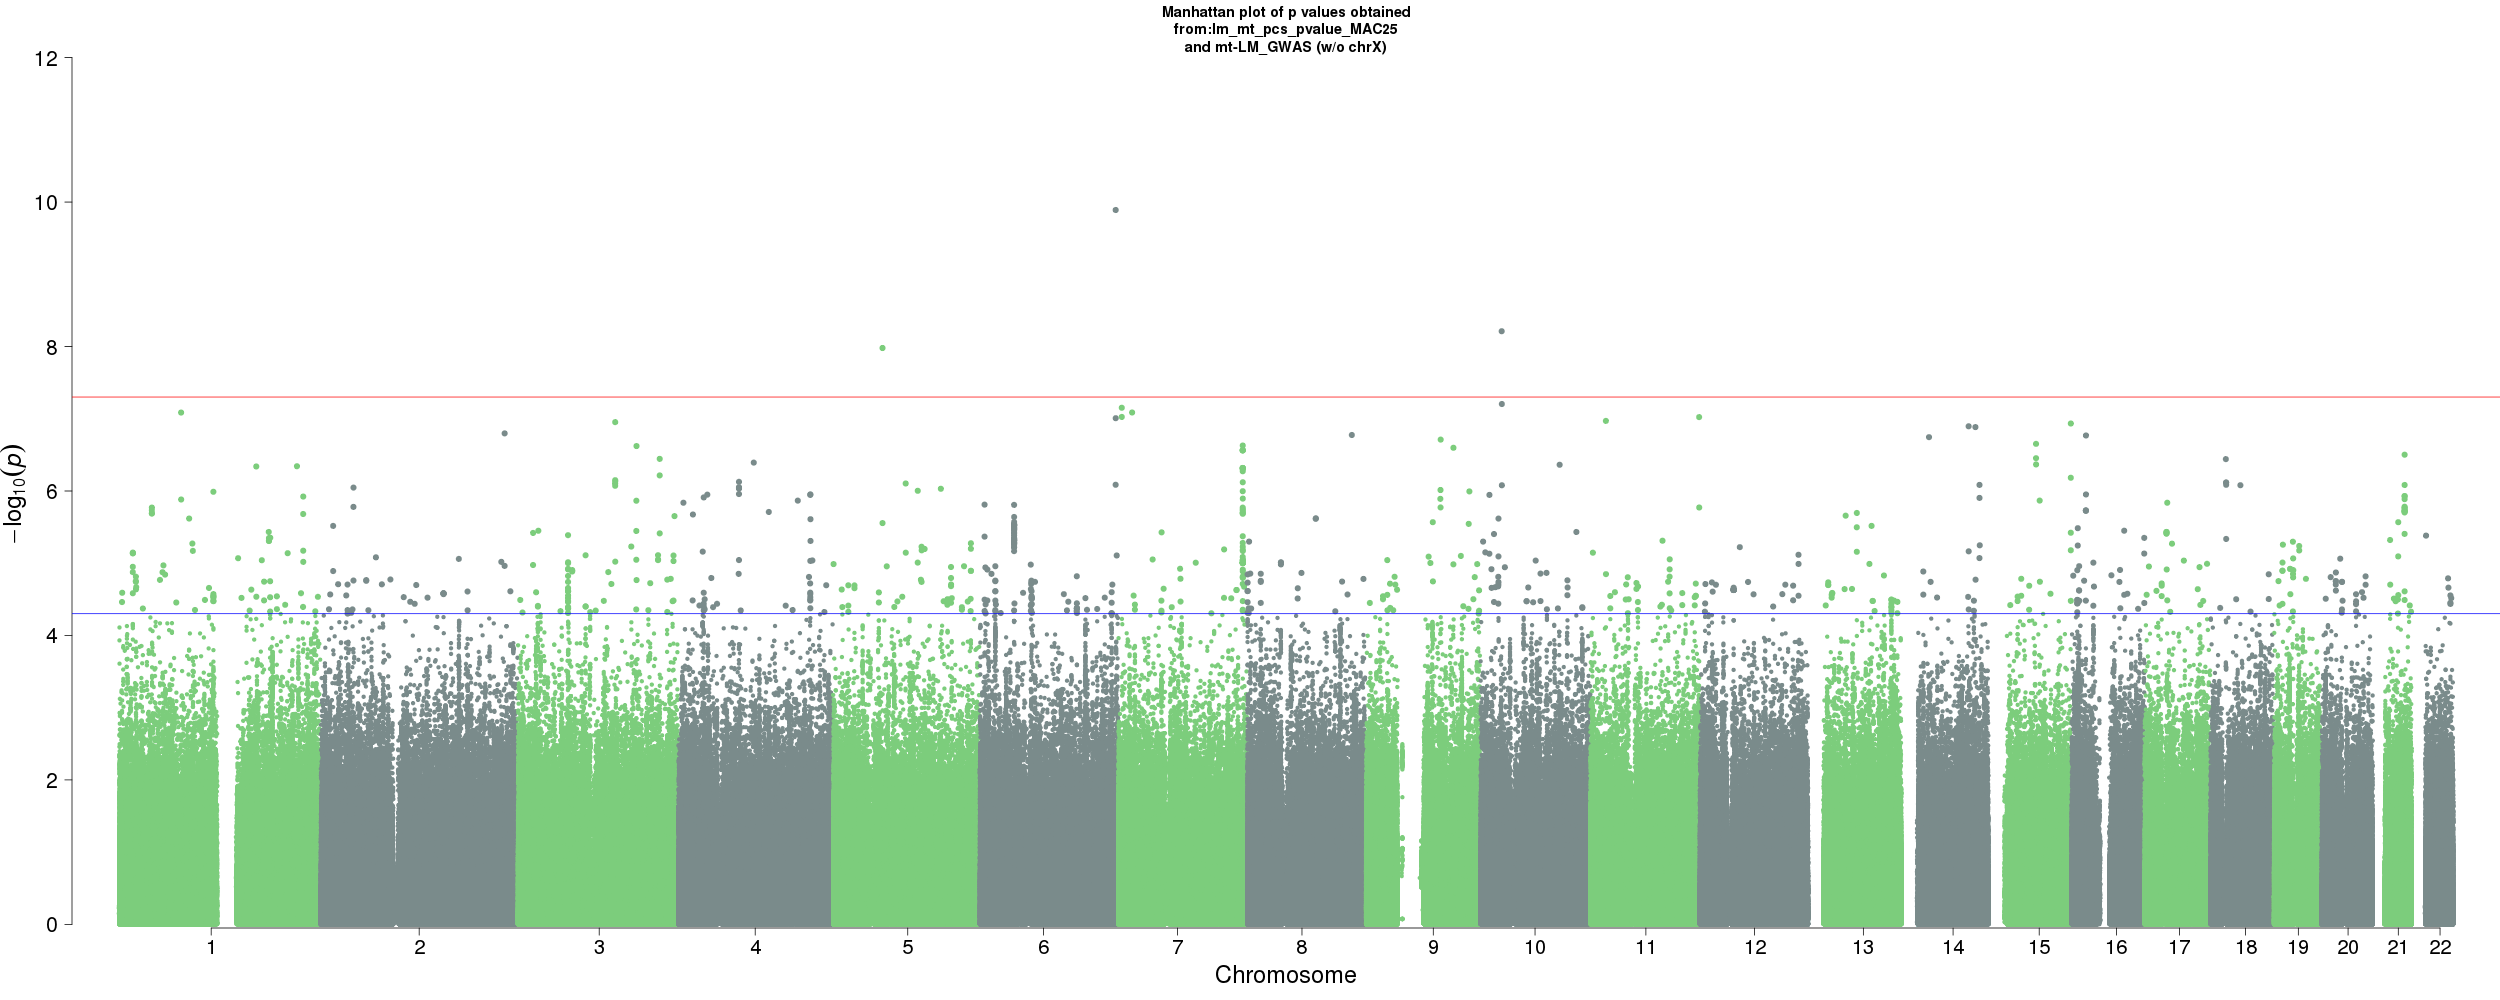
\includegraphics[trim = 0mm 0mm 0mm 60mm, clip, width=1\textwidth]{Figures/lm_mt_pcs_pvalue_MAC25_mt-LM_GWAS_manhattanplot.png}
	\caption{\textbf{Manhattan plot of genome-wide left ventricular wall thickness associations.} All 100 PEER factors were modeled jointly in an any effect mt-LMM-GWAS.}
 	\label{fig:GWAS-pheno3D}
\end{figure}

\subsection{Further work}
\begin{itemize}
\item confirming model calibration by permutations
\item manual QC of genotype cluster plots of SNPs with p-value of less then $5e-4$
\item locus zoom of the genomic regions and biological interpretation
\item replication with UKBiobank data: interpolation of wall thickness measurements from 2d CMR images (access already granted and measurements currently in QC by collaborators)
\end{itemize}
\bibliography{TAC3}
\bibliographystyle{ebi}

\end{document}

